
\documentclass[runningheads]{llncs}
\usepackage[paperheight=295mm,paperwidth=210mm]{geometry}
\usepackage{graphicx}
\usepackage{kotex}
\usepackage[dvipsnames]{xcolor}
\usepackage{fancyvrb}
\usepackage{listings}
\usepackage{indentfirst}
\usepackage{tabularx}
\usepackage{underscore}
\usepackage{multicol}
\usepackage{tikz}
\usepackage[square,sort,comma,super]{natbib}
\usepackage{inconsolata} % Inconsolata
\usepackage{mathptmx} % Times New Roman
\usepackage[cache=false]{minted}
\graphicspath{ {./images/} }
\lstset{basicstyle=\footnotesize\ttfamily,breaklines=true}
\renewcommand{\bibname}{참고문헌}
\setlength{\parindent}{1em}
\setlength{\parskip}{1em}
\linespread{1.2}
{\renewcommand{\arraystretch}{1.5}%
\setlength{\tabcolsep}{0.5em}%
\newenvironment{Figure}
  {\par\medskip\noindent\minipage{\linewidth}}
  {\endminipage\par\medskip}
	
\begin{document}

\title{CSE3013 (컴퓨터공학 설계 및 실험 I) \space \newline WEB-1 결과 보고서}
\author{서강대학교 컴퓨터공학과 박수현 (20181634)}
\institute{서강대학교 컴퓨터공학과}
\maketitle

\section{목적}
실험 과정을 통해서 익힌 HTML을 사용하여 자신의 홈페이지를 직접 제작해 본다.

\section{최소 요구 사항}
\begin{enumerate}
	\item \texttt{frame}을 이용한 메뉴 방식 구조
	\item 자신의 사진을 포함한 프로필(자기 소개) 페이지
	\item 자신의 관심 분야 및 유용한 정보 소개 페이지
	\item 자신의 이번 학기 수강 시간표 페이지(테이블로 작성)
	\item 예비 보고서에서 추가로 조사한 기술을 사용
	\item \texttt{http://cs.sogang.ac.kr/\textasciitilde{}자신의 계정/}으로 초기화면이 나타나야 함.
\end{enumerate}

\section{작성 과정 기술}

\subsection{홈페이지 구조}
% 각 문서 파일과 그들의 링크 구조를 Top-Down 형태로 그리시오
\begin{tikzpicture}[nodes = {draw,align=center}]

\node[draw] (main) at (3.25,2) {\textbf{메인 프레임}\\\texttt{index.html}};

\node[draw] (cv) at (0,0) {\textbf{자기 소개}\\\texttt{main.html}};
\node[draw] (interests) at (3,0) {\textbf{관심 분야 소개}\\\texttt{interests.html}};
\node[draw] (timetable) at (6.5,0) {\textbf{수강 시간표}\\\texttt{timetable.html}};

\draw[<->,draw=black] (main) to (cv);
\draw[<->,draw=black] (main) to (interests);
\draw[<->,draw=black] (main) to (timetable);

\draw[<->,draw=black,in=320,out=220] (timetable) to (cv);
\draw[<->,draw=black] (cv) to (interests);
\draw[<->,draw=black] (interests) to (timetable);
\end{tikzpicture}

\subsection{홈페이지 레이아웃 디자인}
% 메인 페이지의 레이아웃을 간략히 그리고 설명하시오
\begin{Figure}
	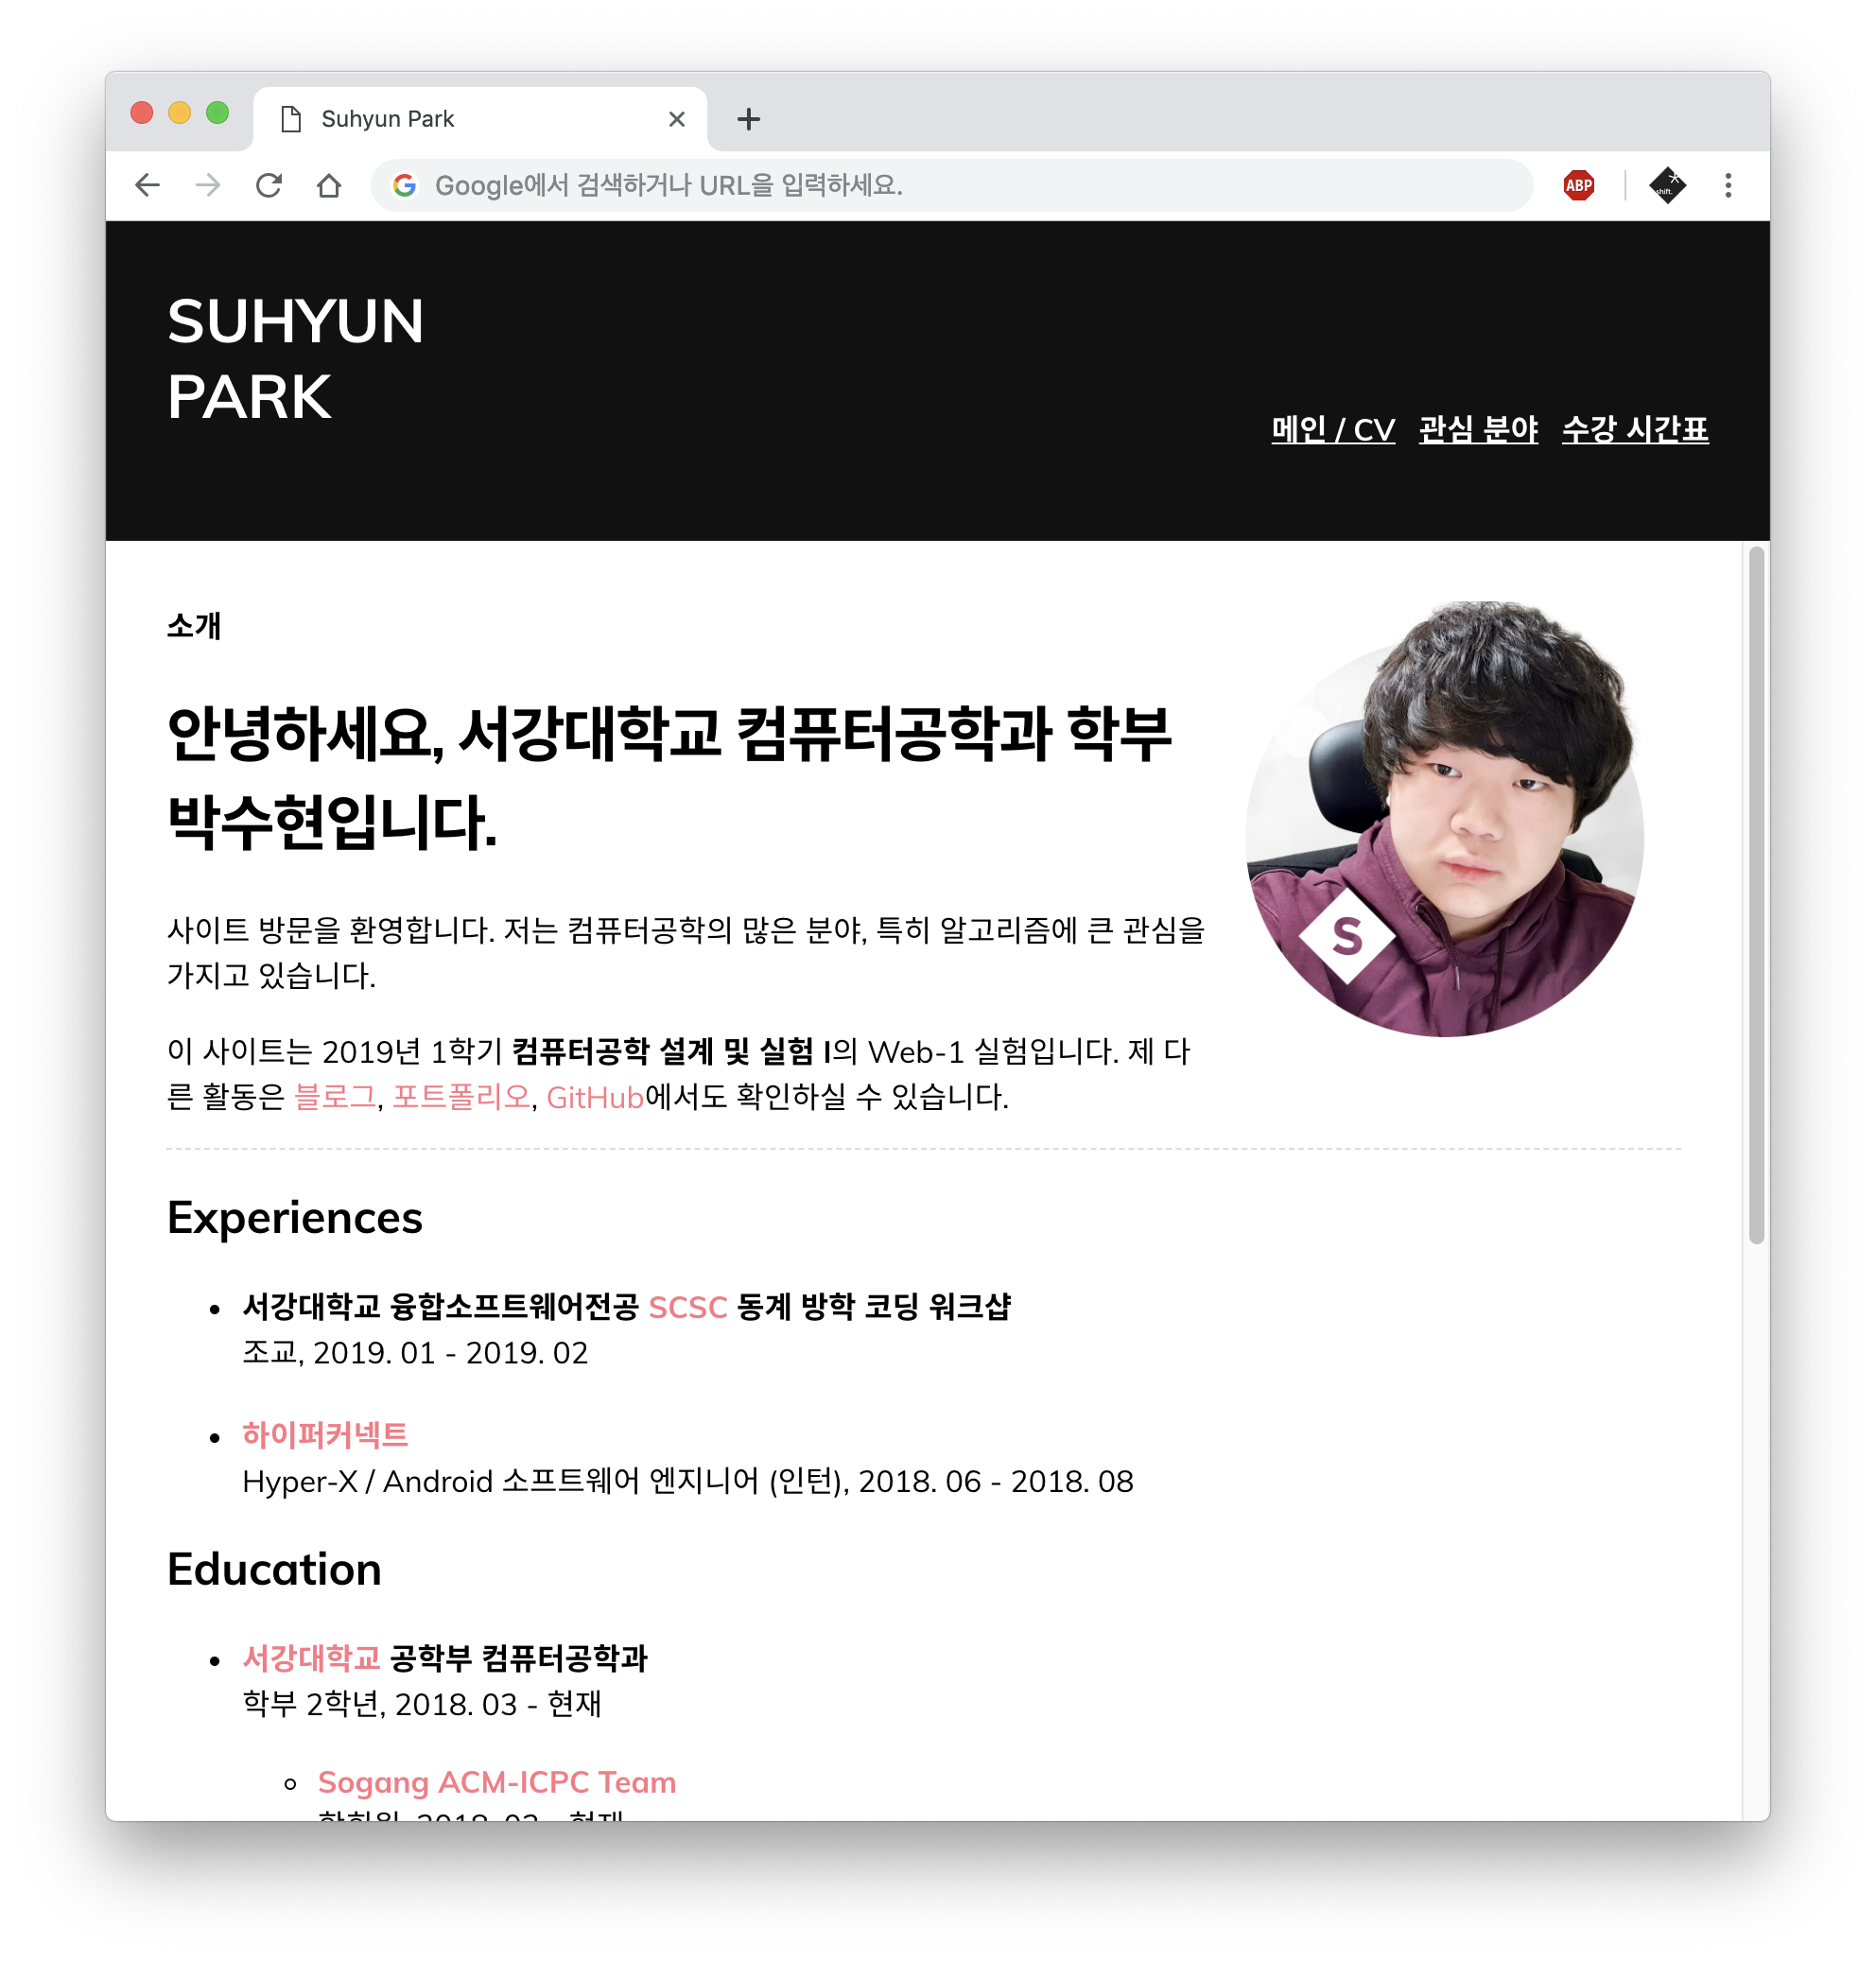
\includegraphics[width=\linewidth]{web-html.png}
	\label{fig:web-html}
\end{Figure}

\begin{itemize}
	\item 페이지는 두 개의 프레임으로 나누었다.
	\item 상단 프레임에는 메뉴를 배치했고, 상단 프레임에서 메뉴 아이템을 클릭하면 하단 프레임의 정보가 바뀌도록 구성하였다. 프레임 윤곽선은 숨겼으며 임의로 크기 조절이 불가능하도록 만들었다.
\end{itemize}


\subsection{HTML 작성 과정}
% 교재에 있는 내용을 자신의 홈페이지에 어떻게 적용하였는지 항목별로 적으시오
실습 교재에 존재하는 내용 중에서 다음과 같은 항목들을 적용하였다.
\begin{itemize}
	\item \texttt{frameset}, \texttt{frame} 태그를 사용해 홈페이지를 구성하였다.
	\item 시간표는 \texttt{table}로 제작하였다. 연강의 경우 셀 여러 개에 걸쳐 표현하지 않고 병합된 하나의 셀 -- \texttt{rowspan}을 이용한 방법 -- 으로 표현하였다.
	\item \texttt{img} 태그를 이용해 이미지를 삽입하였다.
\end{itemize}

% 교재에 없는 내용을 어떻게 적용하였는지 항목별로 적으시오
이외에 임의로 적용된 항목들은 다음과 같다.
\begin{itemize}
	\item CSS 스타일시트와 웹 폰트를 사용해, 웹 사이트를 더욱 보기 좋게 디자인하였다.
	\item 외부 페이지로 이어지는 모든 링크는 \texttt{target} 속성을 이용해 새 탭에서 열리도록 구성했다.
	\item \texttt{viewport} 메타 태그를 이용해 모바일 기기에서도 홈페이지가 자연스럽게 보일 수 있도록 했다.
\end{itemize}

\subsection{정리}
% 기존 유명 홈페이지와 비교하여, 자신의 홈페이지의 장점과 단점을 쓰시오
% 장점
기존 유명 블로깅 플랫폼 등과 비교해 이 실험에서 제작한 홈페이지의 장점으로 다음을 들 수 있을 것이다.
\begin{itemize}
	\item 원치 않는 광고 없이 직접 제작한 컨텐츠만을 방문자에게 제공할 수 있다.
	\item 내용, 배치, 디자인 등의 수정이 완전히 자유롭다.
\end{itemize}

% 단점
한편 다음과 같은 단점도 존재할 것이다.
 \begin{itemize}
	\item \texttt{frame}, \texttt{frameset} 태그는 HTML5 표준에서 더 이상 사용되지 않는(deprecated) 태그이다. 현재는 브라우저들이 \texttt{frame} 태그를 보여주는 데에 문제가 없지만, 표준이 아닌 이상 미래의 브라우저 엔진들은 이 태그를 지원할 필요가 없게 되어 사이트가 정상적으로 보이지 않게 될 여지가 있다. 이 실험에서 만든 것과 같은 메뉴는 \texttt{div} 태그와 CSS \texttt{position: fixed;} 속성을 이용해 구현하는 것이 HTML5 표준에서는 일반적이다.
\end{itemize}

\end{document}
